\documentclass[aspectratio=169]{beamer}  
\usefonttheme{professionalfonts}
\usepackage{xeCJK}
\usepackage{fontspec}
\usepackage{graphicx}
\usepackage{listings}
\usepackage{xcolor}
\usepackage{indentfirst}
\usepackage{tikz}
\usepackage{amssymb}
\usepackage{amsthm}
\usepackage{amsmath}
\usepackage{tabularx}
\usepackage{hyperref}
\usepackage{comment}
\usepackage{ulem}
\usepackage{version}
\usepackage{thmtools}
\usepackage{qtree}
\usepackage{algpseudocode}
\usepackage{mathtools}
\usepackage{multicol}
\usepackage{xcolor}
\usepackage{diagbox}

\usefonttheme[onlymath]{serif}

\XeTeXlinebreaklocale "zh"
\XeTeXlinebreakskip = 0pt plus 1pt

\setsansfont{JetBrainsMono-Medium.ttf}
\setCJKmainfont[AutoFakeBold,AutoFakeSlant]{NotoSansTC-Regular.otf}
\usetikzlibrary{arrows,decorations.markings,decorations.pathreplacing}
\newenvironment{Hint}{\noindent\textbf{Hint.}}{}

\tikzstyle {graph node} = [circle, draw, minimum width=1cm]
\tikzset{edge/.style = {decoration={markings,mark=at position 1 with %
            {\arrow[scale=2,>=stealth]{>}}},postaction={decorate}}}

\lstset{
    language=C++,
    basicstyle=\ttfamily\tiny,
    commentstyle=\color{black!50},
    keywordstyle=\color{white!0!blue},
    stringstyle=\color{black!50!green},
    showspaces=false,
    showstringspaces=false,
    showtabs=false,
    tabsize=4,
    captionpos=b,
    breaklines=true,
    breakatwhitespace=false,
    escapeinside={\%*}{*)},
    morekeywords={*}
}

\AtBeginSection[]{
  \begin{frame}
  \vfill
  \centering
  \begin{beamercolorbox}[sep=8pt,center,shadow=true,rounded=true]{title}
    \usebeamerfont{title}\insertsectionhead\par%
  \end{beamercolorbox}
  \vfill
  \end{frame}
}

\title{進階資料結構 (Advanced Data Structure)}
\author{sam571128}
\date[附中延平競程讀書會]

\usetheme{Madrid}
\usecolortheme{default}
\setbeamertemplate{itemize items}[square]
\setbeamertemplate{enumerate items}[default]
\setbeamertemplate{blocks}[default]

\begin{document}

    %title
    \begin{frame}
        \titlepage
    \end{frame}
    
    \begin{frame}{目錄}
        \begin{itemize}
            \item 離散化
            \item 離線
            \item 線段樹上二分搜
            \item 動態開點線段樹
            \item 持久化線段樹
            \item 更多線段樹題目
        \end{itemize}
    \end{frame}

    \begin{frame}{前言}
        \begin{itemize}
            \item 這堂課前半的時間會先引導至兩種特殊的線段樹
            \item 剩下的時間會講各種例題
            \item 然後各位初選加油!
            \item 現在我這裡早上五點,\sout{然後我今天有兩個段考 + 一個 project,要死掉了}
            \item 今天有資結 midterm,所以講資結來複習
        \end{itemize}
    \end{frame}

    \section{離散化 (Coordinate Compression)}

    \begin{frame}{離散化 (Coordinate Compression)}
        \begin{itemize}
            \item 一開始,我們首先要介紹的是名為「離散化」的技巧
            \item 這個技巧,相信大家在讀書會上學期的課程都已經學習過了
            \item 不過,我們要再來好好講講這個很重要的技巧是什麼
        \end{itemize}
    \end{frame}

    \begin{frame}{離散化 (Coordinate Compression)}
        \begin{itemize}
            \item 首先,先來看一個很簡單的例子
        \end{itemize}
    \end{frame}

    \begin{frame}{離散化 (Coordinate Compression)}
        \begin{block}{\href{https://cses.fi/problemset/task/1145}{CSES - Increasing Subsequence}}
            給你一個 $n$ 項的陣列,請找到這個陣列中的 LIS 長度。
        \end{block}
        \begin{itemize}
            \item<2-> 可以很顯然的列出下面的 DP 式(忘記或不會的要問喔
            $$dp[i] = \max_{j < i, \ a[j] < a[i]} (dp[j] + 1)$$
            \item<3-> 很顯然地可以在 $\mathcal{O}(n^2)$ 的時間做完 
            \item<4-> 太慢了!
        \end{itemize}
    \end{frame}

    \begin{frame}{離散化 (Coordinate Compression)}
        \begin{itemize}
            \item 注意到,其實如果我們從 $i = 1$ 開始進行枚舉
            \item 那其實對於每一個數字,我們都只需要去找對於 $a[j] < a[i]$ 的最大 $dp[j]$
            \item<2-> 要怎麼做呢?
            \item<3-> 用 BIT 存以 $a[j]$ 做結尾的最大答案!
        \end{itemize}
    \end{frame}

    \begin{frame}{離散化 (Coordinate Compression)}
        \begin{center}
            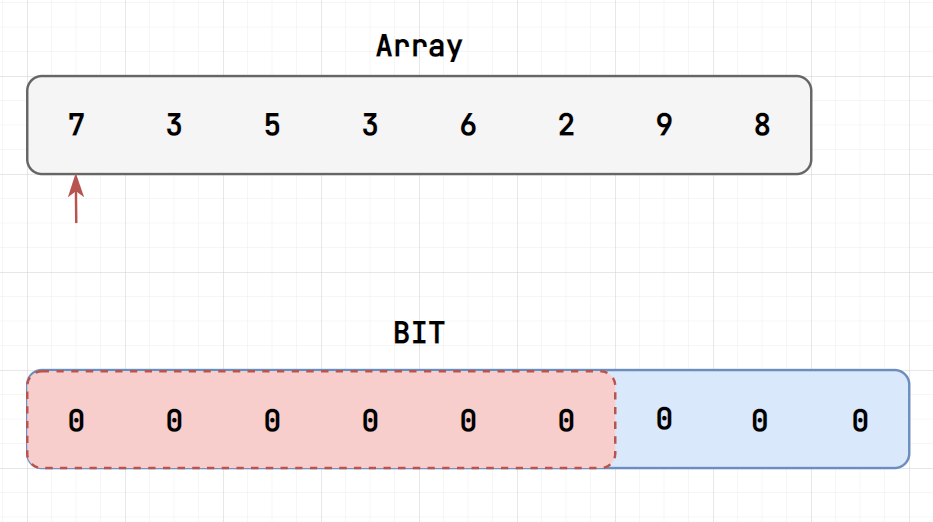
\includegraphics[scale=0.45]{LIS/step1.png}
        \end{center}
    \end{frame}

    \begin{frame}{離散化 (Coordinate Compression)}
        \begin{center}
            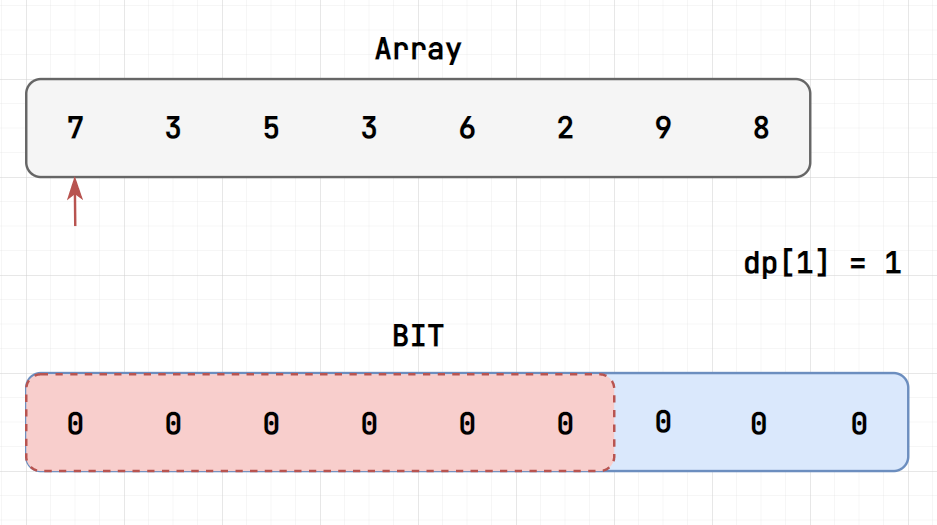
\includegraphics[scale=0.45]{LIS/step2.png}
        \end{center}
    \end{frame}

    \begin{frame}{離散化 (Coordinate Compression)}
        \begin{center}
            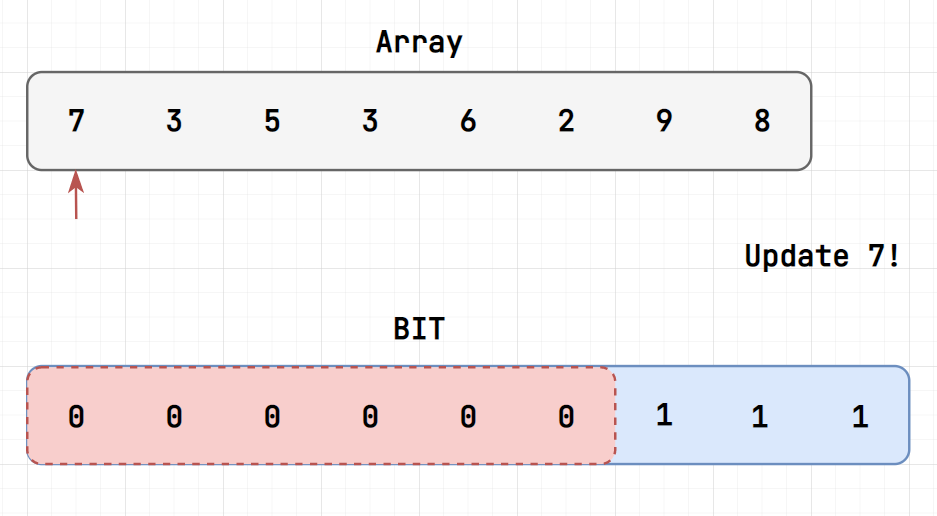
\includegraphics[scale=0.45]{LIS/step3.png}
        \end{center}
    \end{frame}

    \begin{frame}{離散化 (Coordinate Compression)}
        \begin{center}
            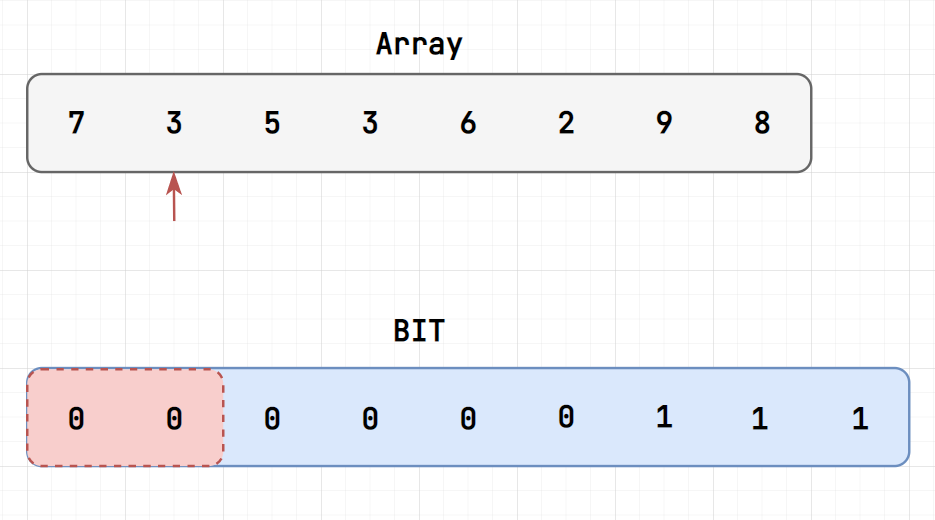
\includegraphics[scale=0.45]{LIS/step4.png}
        \end{center}
    \end{frame}

    \begin{frame}{離散化 (Coordinate Compression)}
        \begin{center}
            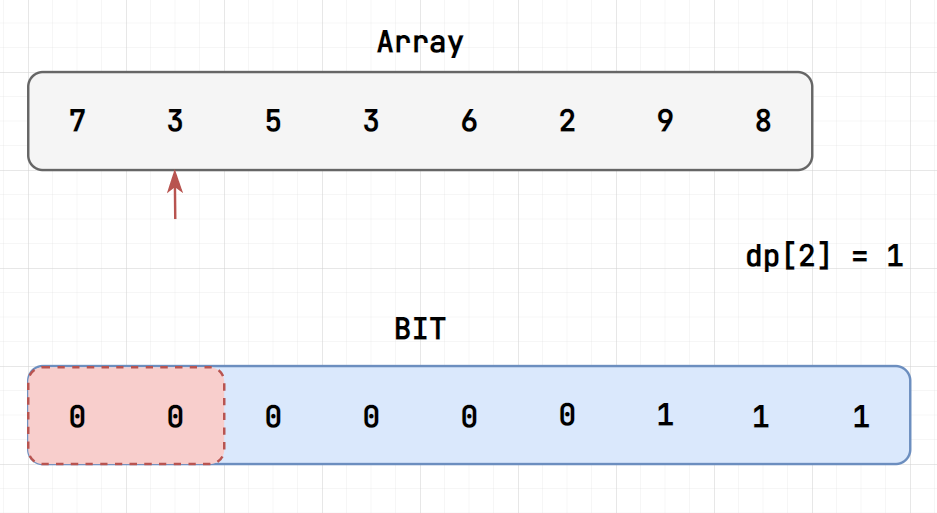
\includegraphics[scale=0.45]{LIS/step5.png}
        \end{center}
    \end{frame}

    \begin{frame}{離散化 (Coordinate Compression)}
        \begin{center}
            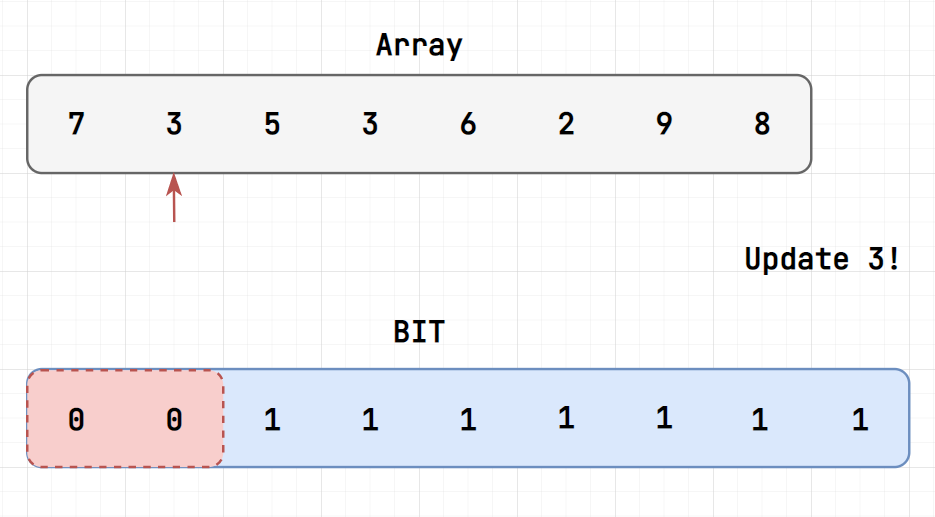
\includegraphics[scale=0.45]{LIS/step6.png}
        \end{center}
    \end{frame}

    \begin{frame}{離散化 (Coordinate Compression)}
        \begin{center}
            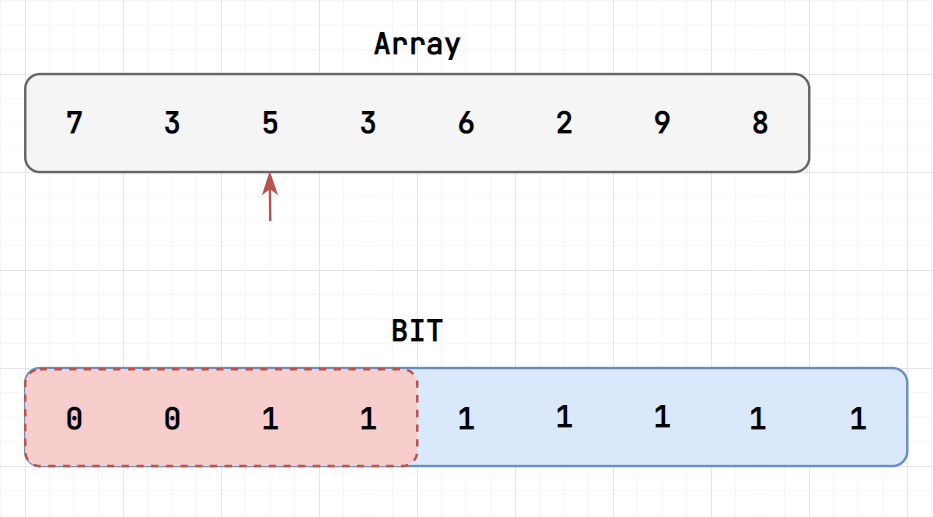
\includegraphics[scale=0.45]{LIS/step7.png}
        \end{center}
    \end{frame}

    \begin{frame}{離散化 (Coordinate Compression)}
        \begin{center}
            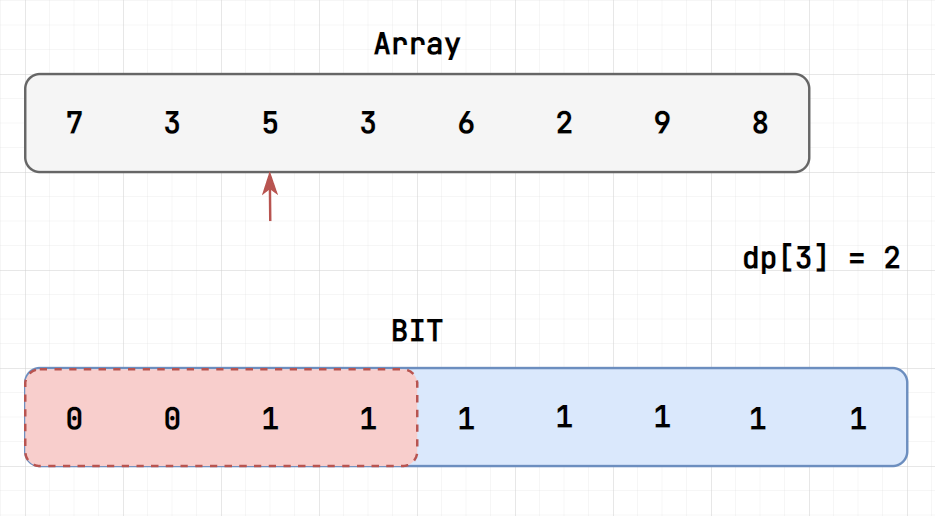
\includegraphics[scale=0.45]{LIS/step8.png}
        \end{center}
    \end{frame}

    \begin{frame}{離散化 (Coordinate Compression)}
        \begin{center}
            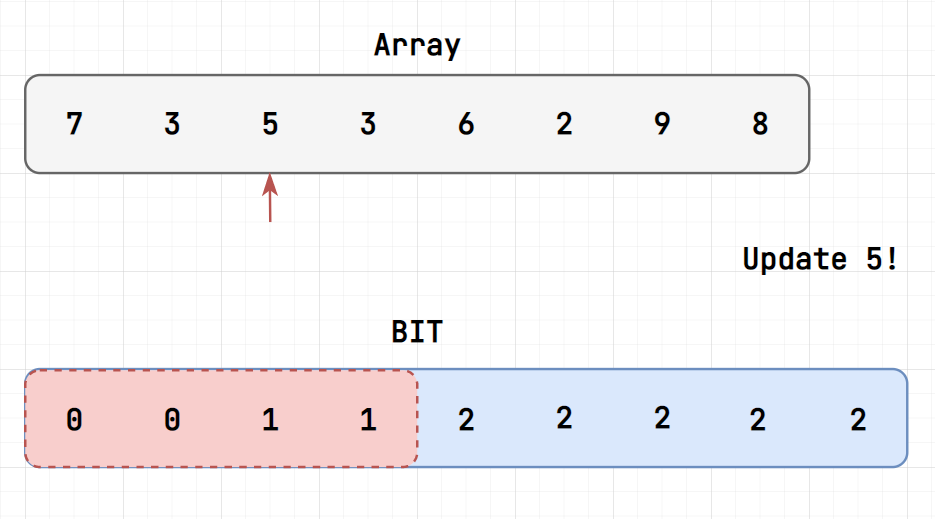
\includegraphics[scale=0.45]{LIS/step9.png}
        \end{center}
    \end{frame}

    \begin{frame}{離散化 (Coordinate Compression)}
        \begin{itemize}
            \item 雖然剛剛那個樣子很合理,但是有沒有注意到什麼事情?
            \item<2-> 我們對於每一個數字,都會在 BIT 上開一個位置給它
            \item<3-> 因此,當 $\max(a_i)$ 很大 ($10^8, 10^9$) 的時候,空間會存不下!
        \end{itemize}
    \end{frame}

    \begin{frame}{離散化 (Coordinate Compression)}
        \begin{itemize}
            \item 注意到其實在做這件事情時,重要的只有大小關係!(找比 $a[i]$ 小的 dp 答案)
            \item 而我們實際上在 BIT 上修改和詢問的位置,其實最多只有 $n$ 個
            \item<2-> 因此,將這些數字進行轉換,讓他們對應到 $1 \sim n$ 之間的數字,保留大小關係
        \end{itemize}
    \end{frame}

    \begin{frame}{離散化 (Coordinate Compression)}
        假設我們將出現的數字排序好,則他們會如下圖一一對應
        \begin{center}
            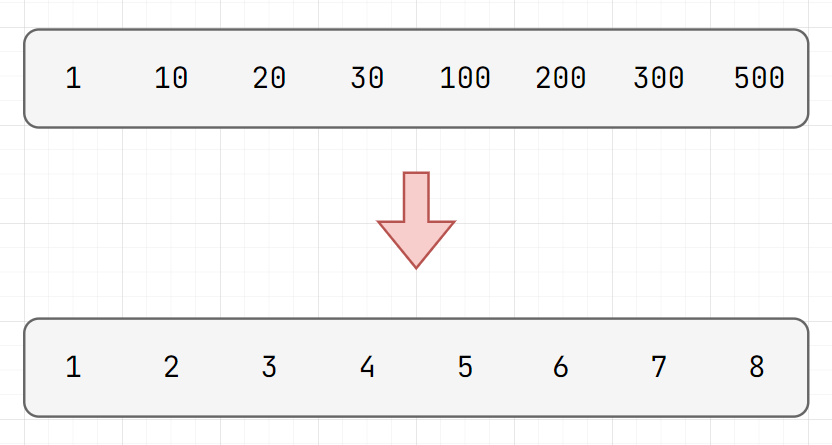
\includegraphics[scale=0.3]{coordinate compression/coordinate_compression.png}
        \end{center}
    \end{frame}

    \begin{frame}{離散化 (Coordinate Compression)}
        \begin{itemize}
            \item 那我們要怎麼做到這一點,有兩種常見的方法
            \begin{enumerate}
                \item 二分搜 (unique + lower\_bound)
                \item map + set
            \end{enumerate}
            \item 第二種方法的常數會比第一種大很多,因此,建議使用第一種
            \vspace{1cm}
            \item<2-> \href{https://cses.fi/paste/7b8182985ab6276b4713df/}{範例 code $\leftarrow$}
        \end{itemize}
    \end{frame}

    \section{離線 (Offline Method)}
    
    \begin{frame}{離線 (Offline Method)}
        \begin{itemize}
            \item 接著,我們要來介紹的技巧為「離線」
            \item 首先,我們先來講講,「離線」是什麼,「在線」又是什麼?
            \item<2-> 兩者的差異:
            \begin{itemize}
                \item 在線:必須照著詢問與操作的順序下去執行
                \item 離線:可以以不同的順序去進行操作
            \end{itemize}
            \item<3-> 第一次聽到可能會不理解兩者差在哪,因此我們實際來看看例題吧
        \end{itemize}
    \end{frame}

    \begin{frame}{離線 (Offline Method)}
        \begin{block}{\href{https://cses.fi/problemset/task/1734/}{CSES - Distinct Value Queries}}
            有一個 $n$ 項的陣列以及 $q$ 筆詢問,每筆詢問請找到區間 $[l,r]$ 內有幾個不同的數字。 \\
            \vspace{0.5cm}
            \begin{itemize}
                \item $1 \le n,q \le 2 \cdot 10^5$
                \item $1 \le a_i \le 10^9$
            \end{itemize}
        \end{block}
        \begin{itemize}
            \item<2-> 乍看之下,應該會發現這題沒有那麼好做(?
            \item<2-> 想法可能會是對線段樹的每個節點開 set 等等的方式去維護
            \item<3-> 不論是時間複雜度$\mathcal{O}(q \log^2 n)$還是空間複雜度都有點太高!
        \end{itemize}
    \end{frame}

    \begin{frame}{離線 (Offline Method)}
        \begin{itemize}
            \item 有沒有什麼辦法,可以讓我們更簡單的處理這個問題?
            \item 假如,一開始你就已經知道有哪些詢問的區間呢?
        \end{itemize}
    \end{frame}

    \begin{frame}{離線 (Offline Method)}
        \begin{itemize}
            \item 考慮將所有的詢問,按照詢問的左界,由大到小排序
        \end{itemize}
        \begin{center}
            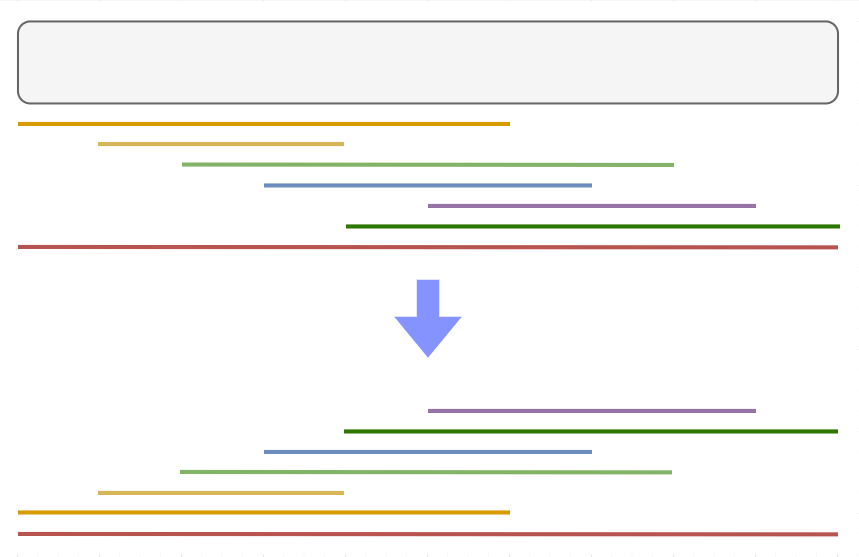
\includegraphics[scale=0.3]{offline/sort_queries.png}
        \end{center}
    \end{frame}

    \begin{frame}{離線 (Offline Method)}
        \begin{itemize}
            \item 思考當我們將左界向左移動時,以 $r$ 當右界的答案會發生什麼事?
        \end{itemize}
        \begin{center}
            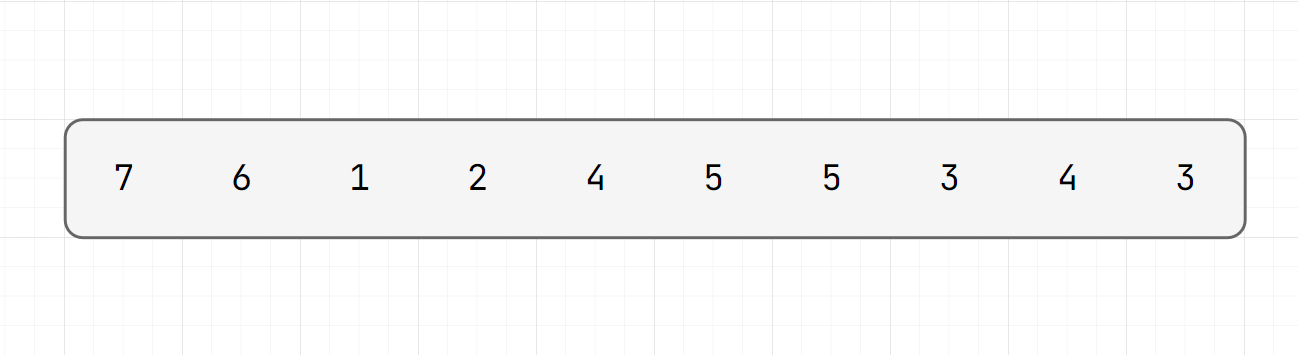
\includegraphics[scale=0.4]{offline/array.png}
        \end{center}
    \end{frame}

    \begin{frame}{離線 (Offline Method)}
        \begin{itemize}
            \item 思考當我們將左界向左移動時,以 $r$ 當右界的答案會發生什麼事?
        \end{itemize}
        \begin{center}
            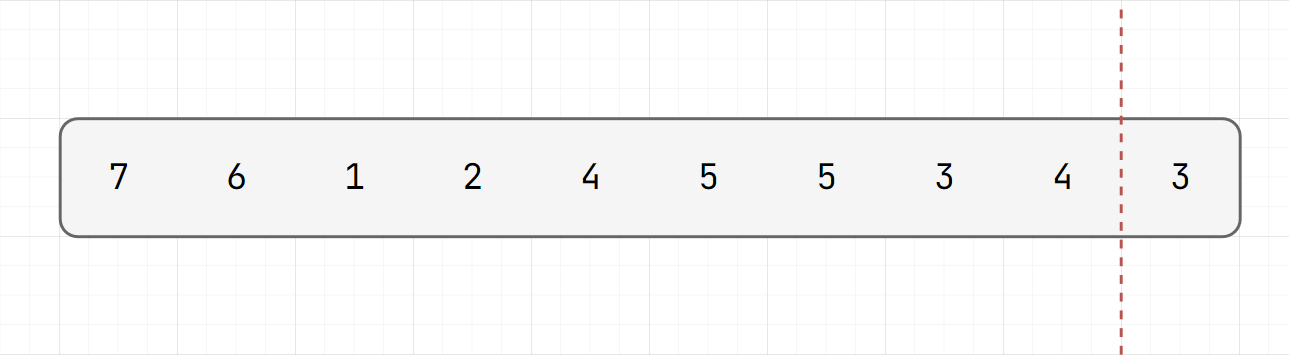
\includegraphics[scale=0.4]{offline/array2.png}
        \end{center}
        \begin{itemize}
            \item $r \in [10,10]$ 的答案會 $+1$!
        \end{itemize}
    \end{frame}

    \begin{frame}{離線 (Offline Method)}
        \begin{itemize}
            \item 思考當我們將左界向左移動時,以 $r$ 當右界的答案會發生什麼事?
        \end{itemize}
        \begin{center}
            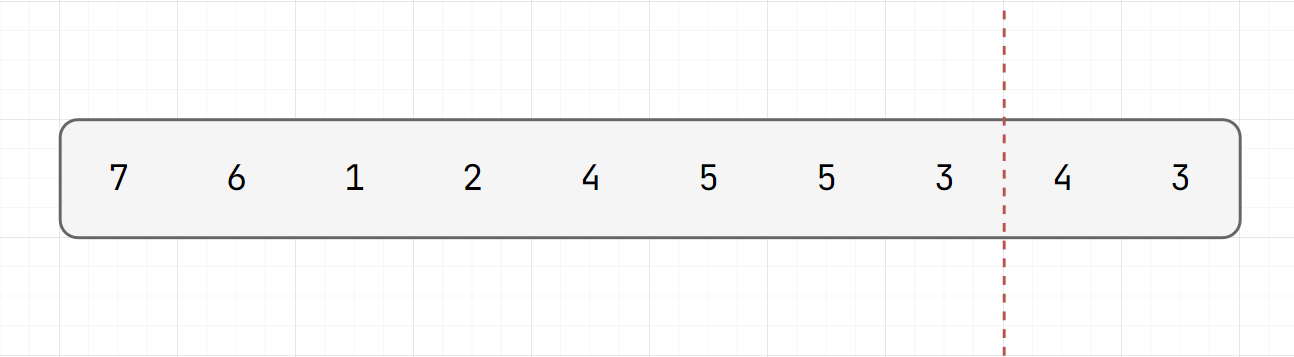
\includegraphics[scale=0.4]{offline/array3.png}
        \end{center}
        \begin{itemize}
            \item $r \in [9,10]$ 的答案會 $+1$!
        \end{itemize}
    \end{frame}

    \begin{frame}{離線 (Offline Method)}
        \begin{itemize}
            \item 思考當我們將左界向左移動時,以 $r$ 當右界的答案會發生什麼事?
        \end{itemize}
        \begin{center}
            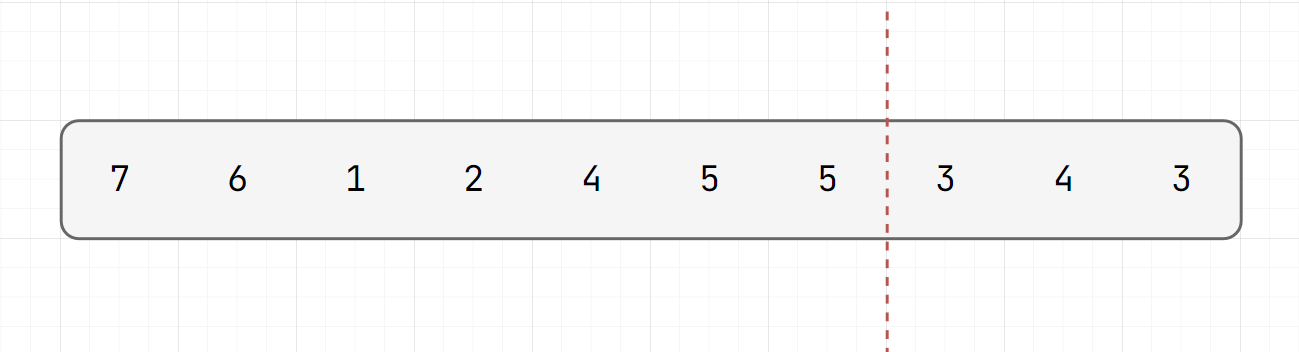
\includegraphics[scale=0.4]{offline/array4.png}
        \end{center}
        \begin{itemize}
            \item $r \in [8,9]$ 的答案會 $+1$!(注意到為什麼是到 $9$ 了嗎?)
        \end{itemize}
    \end{frame}

    \begin{frame}{離線 (Offline Method)}
        \begin{itemize}
            \item 會發現,其實我們真正需要的,只有一個能夠區間加值,單點求和的資料結構
            \item<2-> 這些都是 BIT 或 線段樹 可以做到的!
            \item<3-> 參考程式碼:https://cses.fi/paste/a38a13351d94e2bd316f86/
        \end{itemize}
    \end{frame}

    \section{線段樹上二分搜 (Binary Search on Segment Tree)}

    \begin{frame}{線段樹上二分搜 (Binary Search on Segment Tree)}
        \begin{itemize}
            \item 接著,讓我們同樣來複習另外一個技巧「線段樹上二分搜」(還有 BIT)
            \item 一樣先來看看一個例子
        \end{itemize}
    \end{frame}

    \begin{frame}{線段樹上二分搜 (Binary Search on Segment Tree)}
        \begin{block}{PBDS(?}
            現在,請你維護一個 multiset,可以做到以下四種操作
            \begin{enumerate}
                \item 插入 $x$
                \item 刪除 $x$
                \item 詢問第 $k$ 大的數字是多少 (或 $-1$)
                \item 詢問 $x$ 比集合中多少數字還要大 (第 $k$ 大)
            \end{enumerate}
        \end{block}
    \end{frame}

    \begin{frame}{線段樹上二分搜 (Binary Search on Segment Tree)}
        \begin{itemize}
            \item 對 STL 熟悉的人,應該可以很直接地想到,這不就是 PBDS 的 Tree 嗎?
            \item<2-> 沒有錯! 不過,假設你忘了,而且也不會 Treap 等等的平衡二元樹
            \item<3-> 那我們可以使用 BIT 或線段樹來做到這件事情!
        \end{itemize}
    \end{frame}

    \begin{frame}{線段樹上二分搜 (Binary Search on Segment Tree)}
        \begin{itemize}
            \item 考慮用一棵 BIT 或線段樹去維護每個數字出現的頻率(可能要離散化)
            \item 對於前兩種操作,其實就只是 add(x,1) 和 add(x,-1) 這樣的操作而已
            \item 那麼後兩種操作呢?
        \end{itemize}
    \end{frame}

    \begin{frame}[fragile]{線段樹上二分搜 (Binary Search on Segment Tree)}
        \begin{itemize}
            \item 最直覺的想法:直接另外寫一個二分搜檢查!
            \item 由於第三四種操作概念差不多,我們這裡只示範第三種
        \end{itemize}
        \begin{lstlisting}[language=C++, basicstyle=\ttfamily\small]
    int get(int k){
        int l = 0, r = MAXA;
        while(l < r){
            int mid = l+r>>1;
            if(sum(1,mid) >= k) r = mid;
            else l = mid+1;
        }
    }
        \end{lstlisting}
    \end{frame}

    \begin{frame}[fragile]{線段樹上二分搜 (Binary Search on Segment Tree)}
        \begin{itemize}
            \item 因此,可以在 $O(\log^2 n)$ 做完!
            \item<2-> NO!!!! 太慢了
        \end{itemize}
    \end{frame}

    \begin{frame}[fragile]{線段樹上二分搜 (Binary Search on Segment Tree)}
        \begin{itemize}
            \item 對於 BIT,有一種方法叫做倍增法,可以在 $O(\log n)$ 的時間完成二分搜
            \item 至於正確性,可以想想看 BIT 以 lowbit(i) 作為儲存區間大小來去思考
            \item 範例如下:
        \end{itemize}
        \begin{lstlisting}[language=C++, basicstyle=\ttfamily\small]
    int get(int k){
        int sum = 0, idx = 0;
        for(int i = LOGN; i >= 0; i--){
            if(idx + (1<<i) < MAXN && sum + bit[idx + (1<<i)] < k){
                idx += (1<<i);
                sum += bit[idx];
            }
        }
        return idx+1;
    }
        \end{lstlisting}
    \end{frame}

    \begin{frame}[fragile]{線段樹上二分搜 (Binary Search on Segment Tree)}
        \begin{itemize}
            \item 至於線段樹呢,由於是一棵二元樹
            \item 我們可以根據目前節點的總和,決定要往左還右邊進行 DFS
            \item 直到達到我們要找的數字後終止
        \end{itemize}
        \begin{center}
            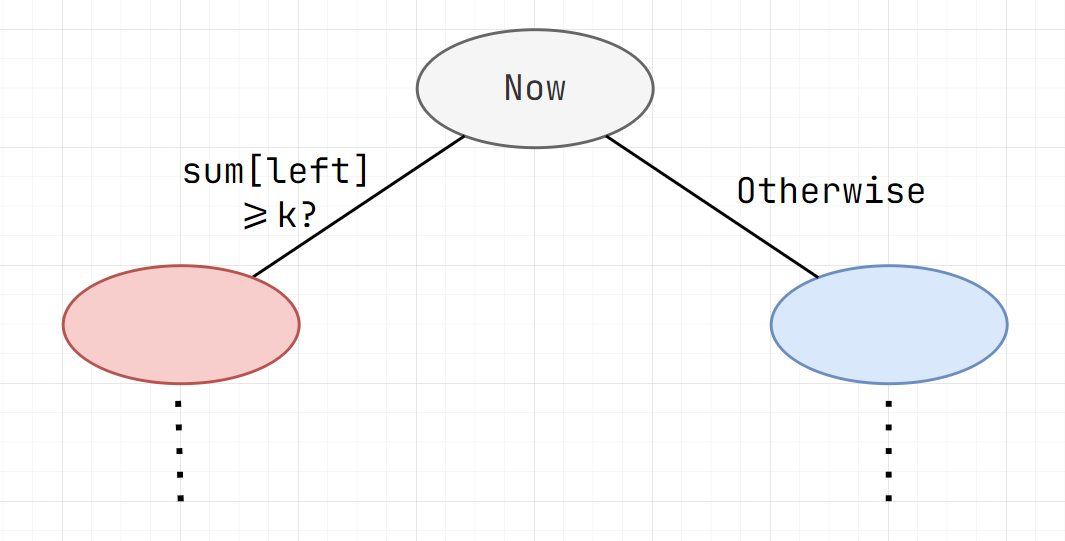
\includegraphics[scale=0.2]{binary_search_on_segment_tree/binary_search_on_segment_tree.png}
        \end{center}
    \end{frame}

    \begin{frame}[fragile]{線段樹上二分搜 (Binary Search on Segment Tree)}
        \begin{itemize}
            \item 這裡不再另外放教學,請回去看 資料結構課的簡報 或者 \href{https://wiki.sam571128.codes/data-structure/segment-tree/segment-tree-2}{山姆的競程維基} 學習
        \end{itemize}
    \end{frame}

    \section{動態開點線段樹 (Dynamic Segment Tree)}

    \begin{frame}{動態開點線段樹 (Dynamic Segment Tree)}
        \begin{itemize}
            \item 終於來到今天的重點之一了,也就是所謂的「動態開點線段樹」(和 BIT)
        \end{itemize}
    \end{frame}

    \begin{frame}{動態開點線段樹 (Dynamic Segment Tree)}
        \begin{itemize}
            \item 在這堂課的最一開始,我們就講到了所謂「離散化」的技巧
            \item 不過,它卻有一個缺點:這個技巧只能用在 \textbf{已知所有詢問} 時
            \item<2-> 因為離散化通常會需要是離線的,只要遇到沒有辦法的題目就會卡住!
        \end{itemize}
    \end{frame}

    \begin{frame}{動態開點線段樹 (Dynamic Segment Tree)}
        \begin{itemize}
            \item 題目通常會用各式各樣的方法來防範你使用「離線的技巧」
        \end{itemize}
        \begin{center}
            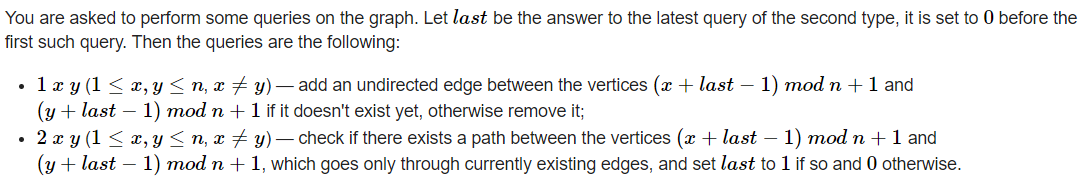
\includegraphics[scale=0.5]{dynamic/Forced_Online_Queries.png}
        \end{center}
        \begin{itemize}
            \item 最常見的即為這種,「下一筆詢問與上一筆詢問的答案有關」的題目
        \end{itemize}
    \end{frame}

    \begin{frame}{動態開點線段樹 (Dynamic Segment Tree)}
        \begin{itemize}
            \item 第二種可能會需要使用到這種線段樹的可能性則為「需要開好多棵」的情況
            \item 經典例題:\href{https://tioj.ck.tp.edu.tw/problems/1169}{TIOJ 1169 - 氣球博覽會}
            \item 假設你今天要開 $10^5$ 棵值域為 $10^5$ 的線段樹 $\Rightarrow$ Explosion!
        \end{itemize}
    \end{frame}

    \begin{frame}{動態開點線段樹 (Dynamic Segment Tree)}
        \begin{itemize}
            \item 看完上述的兩種例子以後,應該能理解離散化所沒辦法做到的原因了吧!
            \item 那麼,我們要怎麼樣讓我們的線段樹有辦法解決這樣的缺點呢?
            \item<2-> 很簡單!用不到的空間,那我們就不要開就好了啊!
            \item<3-> 這裡用一個簡單的例子來看看動態開點的線段樹
        \end{itemize}
    \end{frame}

    \begin{frame}{動態開點線段樹 (Dynamic Segment Tree)}
        \begin{block}{單點加值區間取 min}
            現在有一個 $10^9$ 項的陣列,每個位置都是 $\infty$,有 $q$ 種操作或詢問,每次有兩種可能
            \begin{enumerate}
                \item 對 $arr[x]$ 設成 $v$
                \item 詢問區間 $[l,r]$ 的最小值
            \end{enumerate}
            \vspace{0.5cm}
            \begin{itemize}
                \item $1 \le x \le 10^9$
                \item $1 \le l \le r \le 10^9$
            \end{itemize}
        \end{block}
    \end{frame}

    \begin{frame}{動態開點線段樹 (Dynamic Segment Tree)}
        \begin{itemize}
            \item 一開始的線段樹,會是一個不存在的節點
        \end{itemize}
        \begin{center}
            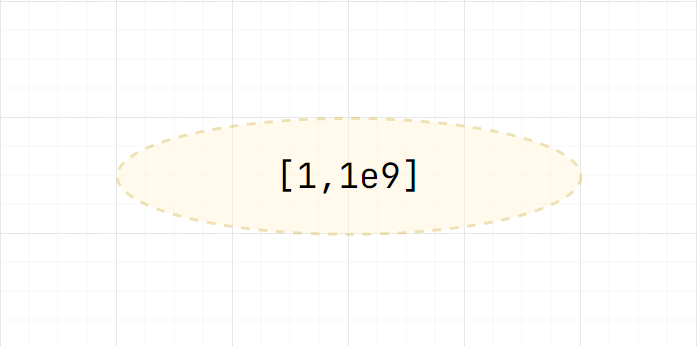
\includegraphics[scale=0.4]{dynamic/initial.png}
        \end{center}
    \end{frame}

    \begin{frame}{動態開點線段樹 (Dynamic Segment Tree)}
        \begin{itemize}
            \item 假設在這個時候,我們詢問 $[1,2]$ 的最小值,由於節點不存在,直接回傳是 $\infty$
        \end{itemize}
        \begin{center}
            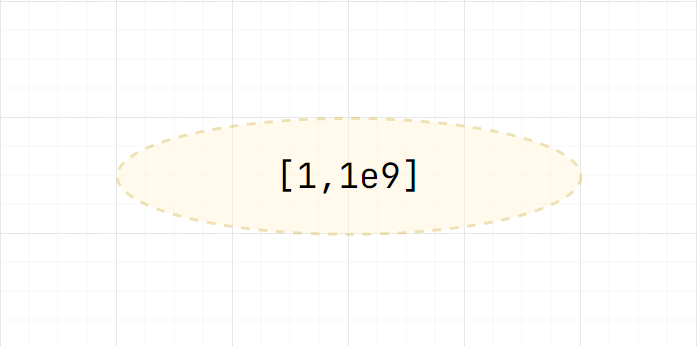
\includegraphics[scale=0.4]{dynamic/initial.png}
        \end{center}
    \end{frame}

    \begin{frame}{動態開點線段樹 (Dynamic Segment Tree)}
        \begin{itemize}
            \item 假設現在,我們對 $arr[1]$ 加 $1$,則我們要新增從根到葉子路徑上的所有點
        \end{itemize}
        \begin{center}
            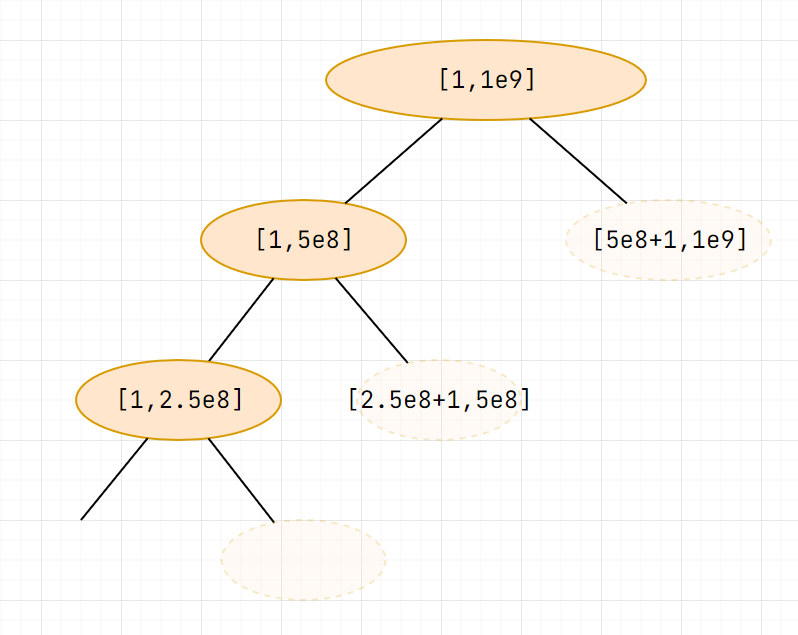
\includegraphics[scale=0.3]{dynamic/add1.png}
        \end{center}
    \end{frame}

    \begin{frame}{動態開點線段樹 (Dynamic Segment Tree)}
        \begin{itemize}
            \item 那當我們這時候要再詢問 $[1,5e8+2]$ 的時候,實際覆蓋到的節點會是這兩個節點
        \end{itemize}
        \begin{center}
            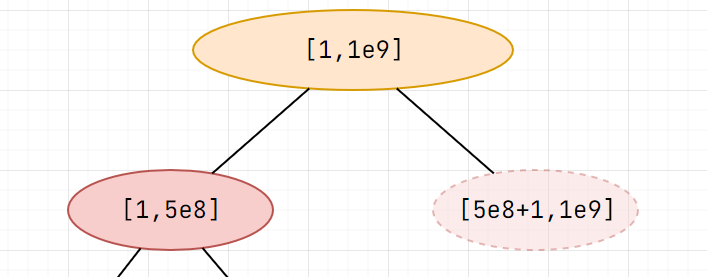
\includegraphics[scale=0.3]{dynamic/ask1.png}
        \end{center}
        \begin{itemize}
            \item 由於右邊的節點預設是 $\infty$ 了,我們不必向下走也能知道那裡的答案會是 $\infty$
            \item 答案取 $[1,5e8]$ 的 $1$ 和 $\infty$ 取 min
        \end{itemize}
    \end{frame}

    \begin{frame}{動態開點線段樹 (Dynamic Segment Tree)}
        \begin{itemize}
            \item 因此,動態開點線段樹的概念就是
            \item 當我們修改時,走到空的點,就新增點
            \item 詢問時,遇到空的點,就直接回傳「初始值」,否則就正常回傳
        \end{itemize}
    \end{frame}

    \begin{frame}{動態開點線段樹 (Dynamic Segment Tree)}
        \begin{itemize}
            \item 而會發現,在每一次修改時,我們最多新增 $\log n$ 個節點
            \item 每次詢問時,與線段樹的詢問依舊相同
            \item<2-> 因此,空間複雜度為 $O(q_1 \log n)$($q_1$ 是修改次數)
            \item<2-> 至於時間複雜度,皆與一般的線段樹相同(不過 $n$ 通常比一般情況大)
            \item<3-> 實作的話建議自己用這概念實作看看,我會在最後附上 code
        \end{itemize}
    \end{frame}

    \begin{frame}{動態開點 BIT!(Dynamic BIT)}
        \begin{itemize}
            \item 你可能會想,那 BIT 可不可以動態開點
            \item<2-> 答案是可以!
        \end{itemize}
    \end{frame}

    \begin{frame}[fragile]{動態開點 BIT!(Dynamic BIT)}
        \begin{itemize}
            \item 思考看看 BIT 的實作方式
        \end{itemize}
        \begin{lstlisting}[language=C++,basicstyle=\ttfamily \small]
    int bit[MAXN];
    void update(int pos, int val){
        while(pos < MAXN){
            bit[pos] += pos;
            pos += pos&-pos;
        }
    }
        \end{lstlisting}
        \begin{itemize}
            \item 有沒有什麼東西可以像陣列一樣使用,但又可以動態開新的空間?
        \end{itemize}
    \end{frame}

    \begin{frame}[fragile]{動態開點 BIT!(Dynamic BIT)}
        \begin{itemize}
            \item 實際上,將 bit 的宣告,從陣列替換成 map, unordered\_map,即可有動態開點的 BIT!
        \end{itemize}
        \begin{lstlisting}[language=C++,basicstyle=\ttfamily \small]
    map<int,int> bit;
    void update(int pos, int val){
        while(pos < MAXN){
            bit[pos] += pos;
            pos += pos&-pos;
        }
    }
        \end{lstlisting}
    \end{frame}

    \begin{frame}[fragile]{動態開點 BIT!(Dynamic BIT)}
        \begin{itemize}
            \item 然而,使用 map, unordered\_map 的 BIT 在實際上並不常用
            \item 實際寫下去之後,你也會發現常常會得到一個 TLE
            \item 因為 map 有額外的 log,unordered\_map 亂戳可能也會戳到重複的
            \item<2-> 有沒有更好的 STL 可以幫我們達到這點呢?
        \end{itemize}
    \end{frame}

    \begin{frame}[fragile]{動態開點 BIT!(Dynamic BIT)}
        \begin{itemize}
            \item 實際上,在 policy based data structure 裡面
            \item 還真的有一個能夠在 $O(1)$ 時間完成詢問的 hash table!
            \item 也就是很有名的 gp\_hash\_table(黑魔法)
            \item 這樣就可以無痛的使用動態開點 BIT 了 (不過空間可能還是會逼你離散化)
            \item 詳細可以參考這篇 cf: https://codeforces.com/blog/entry/60737
        \end{itemize}
    \end{frame}

    \section{持久化線段樹 (Persistent Segment Tree)}

    \begin{frame}{什麼是持久化資料結構 (Persistent Data Structure)?}
        \begin{itemize}
            \item 來看看一個例子
        \end{itemize}
    \end{frame}

    \begin{frame}{什麼是持久化資料結構 (Persistent Data Structure)?}
        \begin{block}{持久化 stack}
            現在你有一個 stack,你希望能夠維護以下幾種操作或詢問
            \begin{enumerate}
                \item 將一個數字 push 進去
                \item 將一個數字 pop 掉
                \item 詢問在第 $k$ 次操作後,stack 的最上方是誰
            \end{enumerate}
        \end{block}
    \end{frame}

    \begin{frame}{什麼是持久化資料結構 (Persistent Data Structure)?}
        \begin{columns}
        \begin{column}{0.2\textwidth}
            假設操作依序為
            \begin{enumerate}
                \item push 1
                \item push 3
                \item push 4
                \item pop
                \item push 5
                \item pop
                \item ask 2
                \item ask 3
                \item ask 1
                \item ask 4
                \item ask 5
            \end{enumerate}
        \end{column}
        \begin{column}{0.6\textwidth}
            \begin{center}
                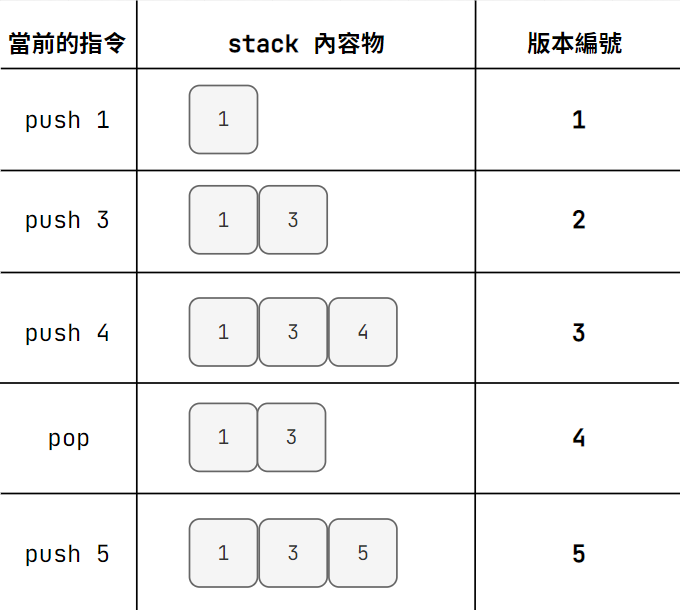
\includegraphics[scale=0.4]{persistent/persistent_stack.png}
            \end{center}
        \end{column}
        \end{columns}
    \end{frame}

    \begin{frame}{什麼是持久化資料結構 (Persistent Data Structure)?}
        \begin{itemize}
            \item 因此,我們只要能夠儲存每一個版本即可
            \item 不過,你會發現,如果要把每一個版本的存起來
            \item 我們的空間又會 Explode!
        \end{itemize}
    \end{frame}

    \begin{frame}{什麼是持久化資料結構 (Persistent Data Structure)?}
        \begin{itemize}
            \item 然而,持久化資料結構其實就是處理這樣情況的一種方式!
        \end{itemize}
    \end{frame}

    \begin{frame}{持久化線段樹 (Persistent Segment Tree)}
        \begin{itemize}
            \item 讓我們回到線段樹的主題,來看看一個最基本的例子
        \end{itemize}
    \end{frame}

    \begin{frame}{持久化線段樹 (Persistent Segment Tree)}
        \begin{block}{\href{https://cses.fi/problemset/task/1737}{CSES - Range Queries and Copies}}
            你現在一個 list,一開始上面只有一個 $n$ 項的陣列,接下來你會進行 $q$ 次三種操作
            \begin{enumerate}
                \item 將 list 上第 $k$ 個陣列設成 $x$
                \item 詢問 list 上第 $k$ 個陣列 $[l,r]$ 區間的和
                \item 將目前的陣列加進 list 的最後面
            \end{enumerate}
        \end{block}
    \end{frame}

    \begin{frame}{持久化線段樹 (Persistent Segment Tree)}
        \begin{itemize}
            \item 應該可以發現這其實跟我們剛剛講的 stack 很像
            \item 不過這前兩個操作其實是線段樹可以做到的操作吧!
            \item<2-> 但是,就跟剛剛講的一樣,你最多有可能存 $q$ 個長度為 $n$ 的陣列
            \item<2-> 當 $n$ 很大時,根本就連空間都開不下阿! 
        \end{itemize}
    \end{frame}
    
    \begin{frame}{持久化線段樹 (Persistent Segment Tree)}
        \begin{itemize}
            \item 仔細思考看看線段樹修改的過程
        \end{itemize}
        \begin{center}
            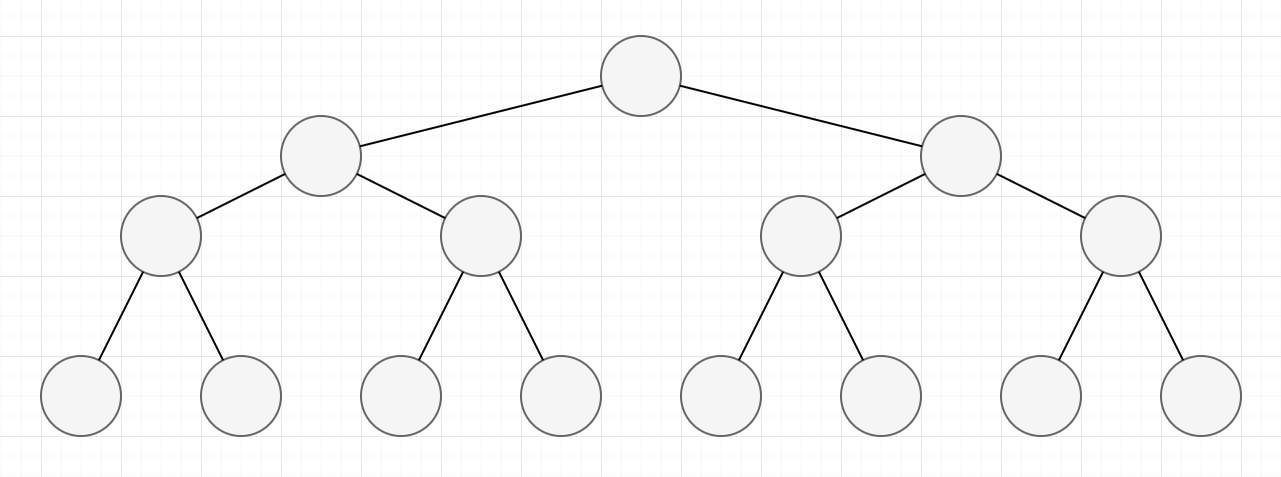
\includegraphics[scale=0.4]{persistent/segment_tree.png}
        \end{center}
    \end{frame}

    \begin{frame}{持久化線段樹 (Persistent Segment Tree)}
        \begin{itemize}
            \item 仔細思考看看線段樹修改的過程
        \end{itemize}
        \begin{center}
            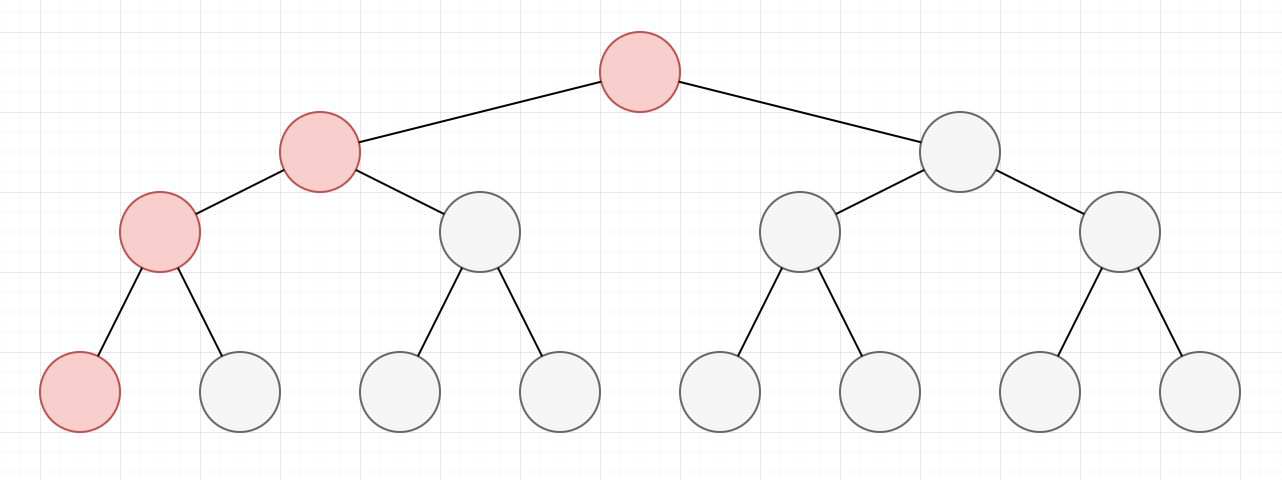
\includegraphics[scale=0.4]{persistent/segment_tree_modify.png}
        \end{center}
    \end{frame}

    \begin{frame}{持久化線段樹 (Persistent Segment Tree)}
        \begin{itemize}
            \item 有沒有發現其實我們只會改到 $\log n$ 個節點,而其他根本不會被改變!
        \end{itemize}
        \begin{center}
            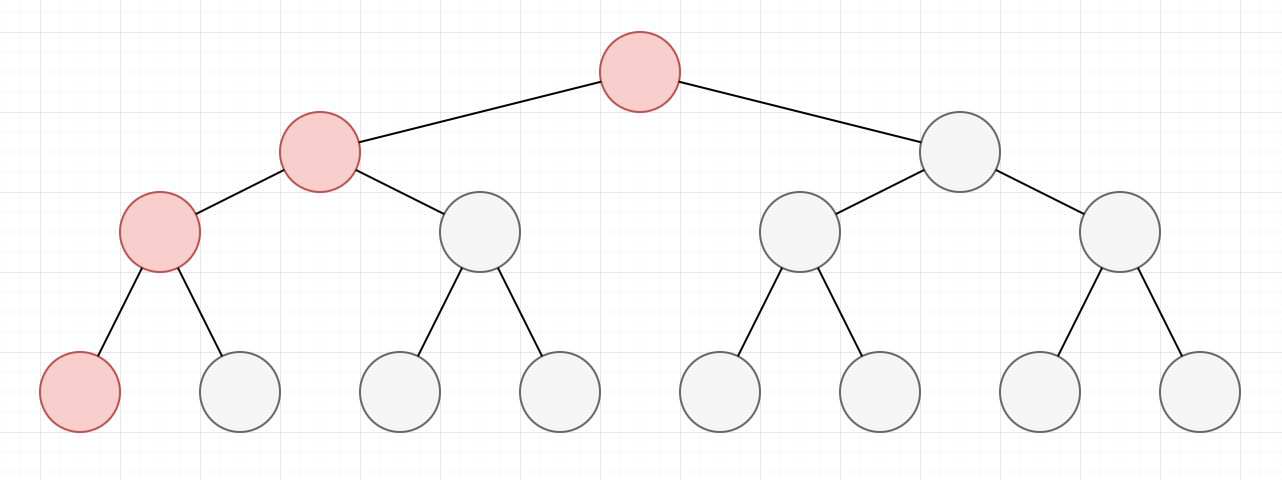
\includegraphics[scale=0.4]{persistent/segment_tree_modify.png}
        \end{center}
    \end{frame}

    \begin{frame}{持久化線段樹 (Persistent Segment Tree)}
        \begin{itemize}
            \item 與動態開點的概念相同,當我們修改一個節點時,我們就開一個新的點
            \item 而新的點如果右節點或左節點沒被修改,就讓它連接到舊的版本(共用)
        \end{itemize}
        \begin{center}
            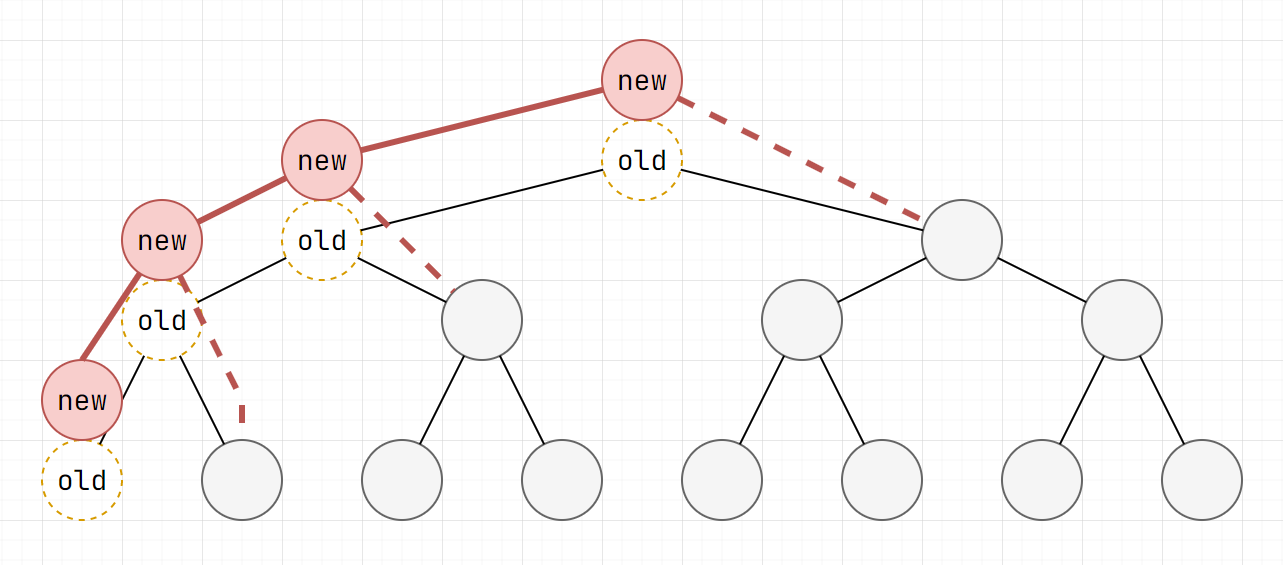
\includegraphics[scale=0.4]{persistent/persisten_segment_tree.png}
        \end{center}
    \end{frame}

    \begin{frame}{持久化線段樹 (Persistent Segment Tree)}
        \begin{itemize}
            \item 這個概念可能對與指標不熟的人來說有點難理解
            \item 不過可以想成,左右孩子原本是連接到 $\texttt{idx}*2$ 和 $\texttt{idx}*2+1$ 的
            \item 但現在,連接的可以是不同編號的,甚至是和其他線段樹共用這些節點
        \end{itemize}
    \end{frame}

    \begin{frame}{持久化線段樹 (Persistent Segment Tree)}
        \begin{itemize}
            \item 我們實際來看 code 解釋一次吧
            \item \href{https://cses.fi/paste/b6682237eee12f582b9ad4/}{範例 code} $\Leftarrow$
        \end{itemize}
    \end{frame}

    \begin{frame}{持久化線段樹 (Persistent Segment Tree)}
        \begin{itemize}
            \item 有了持久化線段樹後的我們能夠做什麼呢?
            \item 事實上,我們現在可以解決原本要離線才能解決的問題了!
        \end{itemize}
    \end{frame}

    \begin{frame}{持久化線段樹 (Persistent Segment Tree)}
        \begin{block}{CSES - Distinct Value Queries (強制在線板)}
            有一個 $n$ 項的陣列以及 $q$ 筆詢問,每筆詢問請找到區間 $[l,r]$ 內有幾個不同的數字。 \\
            \vspace{0.5cm}
            \begin{itemize}
                \item $1 \le n,q \le 2 \cdot 10^5$
                \item $1 \le a_i \le 10^9$
            \end{itemize}
        \end{block}
        \begin{itemize}
            \item<2-> 應該會發現,其實我們可以模仿我們在離線時的做法
            \item<3-> 我們可以在一開始,就將所有左界的線段樹版本給建出來(與離線相同)
            \item<4-> 接著,每次我們就可以直接去取用左界為 $l$ 的版本,詢問 $r$ 的值了!
        \end{itemize}
    \end{frame}

    \begin{frame}{持久化線段樹 (Persistent Segment Tree)}
        \begin{block}{區間第 $k$ 大}
            給你一個 $n$ 項的陣列,接下來有 $q$ 筆詢問,每次請找到區間 $[l,r]$ 中第 $k$ 大的數字\\
            \vspace{0.5cm}
            \begin{itemize}
                \item $1 \le n,q \le 2 \cdot 10^5$
                \item $1 \le a_i \le 10^9$
            \end{itemize}
        \end{block}
    \end{frame}

    \begin{frame}{持久化線段樹 (Persistent Segment Tree)}
        \begin{itemize}
            \item 考慮一個簡單一點的問題,假設你今天想要找陣列 $[1,r]$ 第 $k$ 大的數字,你會怎麼做?
            \item<2-> 前面才剛講過的「線段樹上二分搜」!
        \end{itemize}
    \end{frame}

    \section{更多例題}

    \begin{frame}{?}
        \begin{itemize}
            \item 在這之後的題目,我整理了各種類型的題目給大家做練習
            \item 我會口頭上與大家講這些題目的做法
        \end{itemize}
    \end{frame}

    \begin{frame}{欸? 這看起來是不是就要持久化阿}
        \begin{block}{\href{https://atcoder.jp/contests/abc273/tasks/abc273_e}{AtCoder Beginner Contest 273 E - Notebook}}
            你現在手上有一個 stack 和一本筆記本,接下來有四種操作
            \begin{enumerate}
                \item 將 $x$ 推進 stack
                \item 將 stack 最上面的數字 pop 掉
                \item 將現在的 stack 紀錄在筆記本的第 $y$ 頁
                \item 把手上的 stack 替換成筆記本第 $z$ 頁的 stack
            \end{enumerate}
        \end{block}
    \end{frame}

    \begin{frame}{蝦 不是建一棵線段樹就做完了嗎}
        \begin{block}{\href{https://atcoder.jp/contests/abc273/tasks/abc273_e}{AtCoder Beginner Contest 273 E - Notebook}}
            你現在手上有一個 stack 和一本筆記本,接下來有四種操作
            \begin{enumerate}
                \item 將 $x$ 推進 stack
                \item 將 stack 最上面的數字 pop 掉
                \item 將現在的 stack 紀錄在筆記本的第 $y$ 頁
                \item 把手上的 stack 替換成筆記本第 $z$ 頁的 stack
            \end{enumerate}
        \end{block}
    \end{frame}

    \begin{frame}{蝦 不是建一棵線段樹就做完了嗎}
        \begin{block}{\href{https://tioj.ck.tp.edu.tw/problems/1872}{TIOJ 1872 - 最小公倍數}}
            給你一個陣列,每次詢問請輸出區間 $[l,r]$ 的最小公倍數 $\mod 10^9+7$ 後的結果\\
            \vspace{0.5cm}
            \begin{itemize}
                \item $1 \le n,q \le 10^6$
                \item $1 \le c_i \le 10^6$
            \end{itemize}
        \end{block}
    \end{frame}

    \begin{frame}{剛剛那題的強制在線?}
        \begin{block}{\href{https://codeforces.com/problemset/problem/1422/F}{Codeforces 1422F - Boring Queries}}
            給你一個陣列,每次詢問請輸出區間 $[l,r]$ 的最小公倍數 $\mod 10^9+7$ 後的結果 (強制在線)\\
            \vspace{0.5cm}
            \begin{itemize}
                \item $1 \le n,q \le 10^6$
                \item $1 \le c_i \le 10^6$
            \end{itemize}
        \end{block}
    \end{frame}

    \begin{frame}{蛤 這題要怎麼做 R}
        \begin{block}{\href{https://cses.fi/problemset/task/1664}{CSES - Movie Festival Queries}}
            有 $n$ 部電影,每部電影的播映時間為 $[a_i,b_i]$. 有 $q$ 筆詢問,每次輸出從時間 $l_i$ 到時間 $r_i$ 一共可以完整看完幾部電影\\
            \vspace{0.5cm}
            \begin{itemize}
                \item $1 \le n,q \le 2 \cdot 10^5$
                \item $1 \le a < b \le 10^6$
            \end{itemize}
        \end{block}
    \end{frame}

    \begin{frame}{超級超級經典題!!!}
        \begin{block}{IOI 2014 - Wall}
            你有 $n$ 面牆,接下來你要做 $q$ 個操作,一共有兩種操作
            \begin{enumerate}
                \item 將區間 $[l,r]$ 高度不到 $x$ 的牆高度提升至 $x$
                \item 將區間 $[l,r]$ 高度超過 $x$ 的牆高度降低至 $x$
            \end{enumerate}
            請在最後輸出所有牆的高度
        \end{block}
    \end{frame}

    \begin{frame}{欸? 困難版的 Wall?}
        \begin{block}{111 學年 薇閣高中校內賽 - pG}
            某天,山姆決定要來整理電腦中的檔案。在某個資料夾中,一共有 $n$ 個檔案排成一列,每個檔案的名稱有 $a_i$ 個字。

            接下來,山姆會對這些檔案進行一些操作。
            
            \begin{enumerate}
            \item 將區間 $[l,r]$ 的檔案依照名稱長度\textbf{由小到大排序}
            \item 將區間 $[l,r]$ 的檔案依照名稱長度\textbf{由大到小排序}
            \item 將區間 $[l,r]$ 檔案名稱長度不到 $x$ 的,增加到 $x$
            \item 將區間 $[l,r]$ 檔案名稱長度超過 $x$ 的,減少到 $x$
            \end{enumerate}
            
            在整理過後,他希望能夠知道有哪些位置的檔案名稱長度會是 $k$,請你幫他解決這個問題。
        \end{block}
    \end{frame}
    
\end{document}